\documentclass[12pt, git, final]{rureport}


\begin{document} % this tells the compiler that it is time to make
                 % text to print instead of just getting ready.
\maketitle  % make a title page from the Title, Date, and Author

%\fxnote{skoða titil á skýrslu, sbr. forsíðu}

%\section*{Errata} %%section* avoids putting a number 

\section{Inngangur} % sections break up the document into pieces

Hópverkefni 2 gengur út á það að fara inn á síðuna http://grouplens.org/datasets/movielens/ og ná þar í gagnasett sem inniheldur 10 milljón einkunnargjafir, 100 þúsund 'tags' á 10 þúsund myndum frá 72 þúsund notendum.
\newline
Nemendur eiga svo að skrifa python forrit sem tala við postgresqsl sem geymir MovieLens gagnagrunninn. Forritið á að virka á þann hátt að þegar notandi slær inn heiti á kvikmynd þá á einhvern máta á að birtast notandanum viðbótarupplýsingar þar sem stungið er upp á sambærilegum myndum og myndinni sem var slegin inn í upphafi í forritið.
\newline
\newline
Fljótlega og við byrjuðum að hefjast handa þá vildum við útfæra forritið okkur með graphical user interface til að hafa þetta snyrtilegt og eins 'user friendly' og við gátum á þessum stutta tíma sem nemendur höfðu til að klára verkefnið.
\section{Framkvæmd}
Byrjað var að taka minna gagnasettið sem inniheldur "aðeins" 100 þúsund einkunnargjafir á 1700 kvikmyndum og unnið með hann í byrjun áður en farið var að ná í stærra gagnasettið.
\begin{itemize} 
	\item Fyrst var náð í minna gagnasettið á http://grouplens.org/datasets/movielens/ sen innheldur 100 þúsund einkunnargjafir á 1700 kvikmyndum og unnið með það til að byrja með.
	\item Við lesum inn 3 skrár og setjum movieId sem index.
	\item Splittum dálkinum upp sem er bæði með ár og titil.
	\item 
	\item 
\end{itemize}
 
\section{Hönnun}
Það var ákveðið að hafa GUI mjög einfalt en notendavænt því var búinn til sprettigluggi (sjá mynd \ref{fig:cdbf}), sá gluggi hefur 2 dálka, eina leitarstiku og 5 takka. Til að búa til og hanna graphical user interface var notast við Qt4 designer sem kemur í "app store" á linux kerfinu, það var valið með þeim áherslum að það var auðvelt í notkun og ekki þurfti að forrita alla valmöguleikana heldur var hægt að draga til kassa til að hanna GUI. Krill Krill þú skrifar kannski meira 

\section{Niðurstöður}\label{nidurstodur}
\subsection {Virkni}
Til að sem flestir gætu notað þetta, þá er möguleiki og nokkuð öruggt að gagnagrunnurinn heitir ekki það sama hjá tölvunotendunum og eða allir noti sama lykilorð til að komast inn í hann og því var gripið til þess ráðs að við gætum ýtt á á takka og þá myndi opnast lítill sprettigluggi þar sem nafnið á grunninum og lykilorð væru skrifuð inn til þess að geta tengt forritið við tölvuna (sjá mynd \ref{fig:dbf}).
Eftir að búið er að slá inn viðeigandi upplýsingar (sjá mynd \ref{fig:dbf2}) þá er hægt að ýta á 'test connection' hnappinn og ef upplýsingarnar eru rétt slegnar inn þá birtist annar sprettigluggi sem lætur notendan vita að tenging við gagnagrunn hafi tekist (sjá mynd \ref{fig:pdf3}), hinsvegar ef notandin slær inn vitlausar upplýsingar þá birtist annar sprettigluggi með upplýsingum að tenging hafi mistekist (sjá mynd \ref {fig:dbf3}).
\newline
\newline
Þegar notandinn er búinn að ná að tengjast gagnagrunni þá getur hann skrifað þá mynd sem hann leitar eftir í leitarstikuna (sjá mynd \ref{fig:dbf4}) og ýtir svo á search, niðurstöðurnar birtast svo í vinstri dálknum (sjá mynd \ref{fig:dbf5}) ef notendanum líst svo á einhverja mynd sem kom upp við leitina  getur hann bætt henni við á listan yfir myndir sem hann vill velja, með því að ýta á á 'add' hnappinn og þá dettur myndin í vinstri dálkinn (sjá mynd \ref{fig:dbf6}), þegar ýtt er svo á done þá poppar upp annar spretti gluggi sem kemur með myndir sem þér líkar við. 

\pagebreak
\begin{figure}
	\centering 
	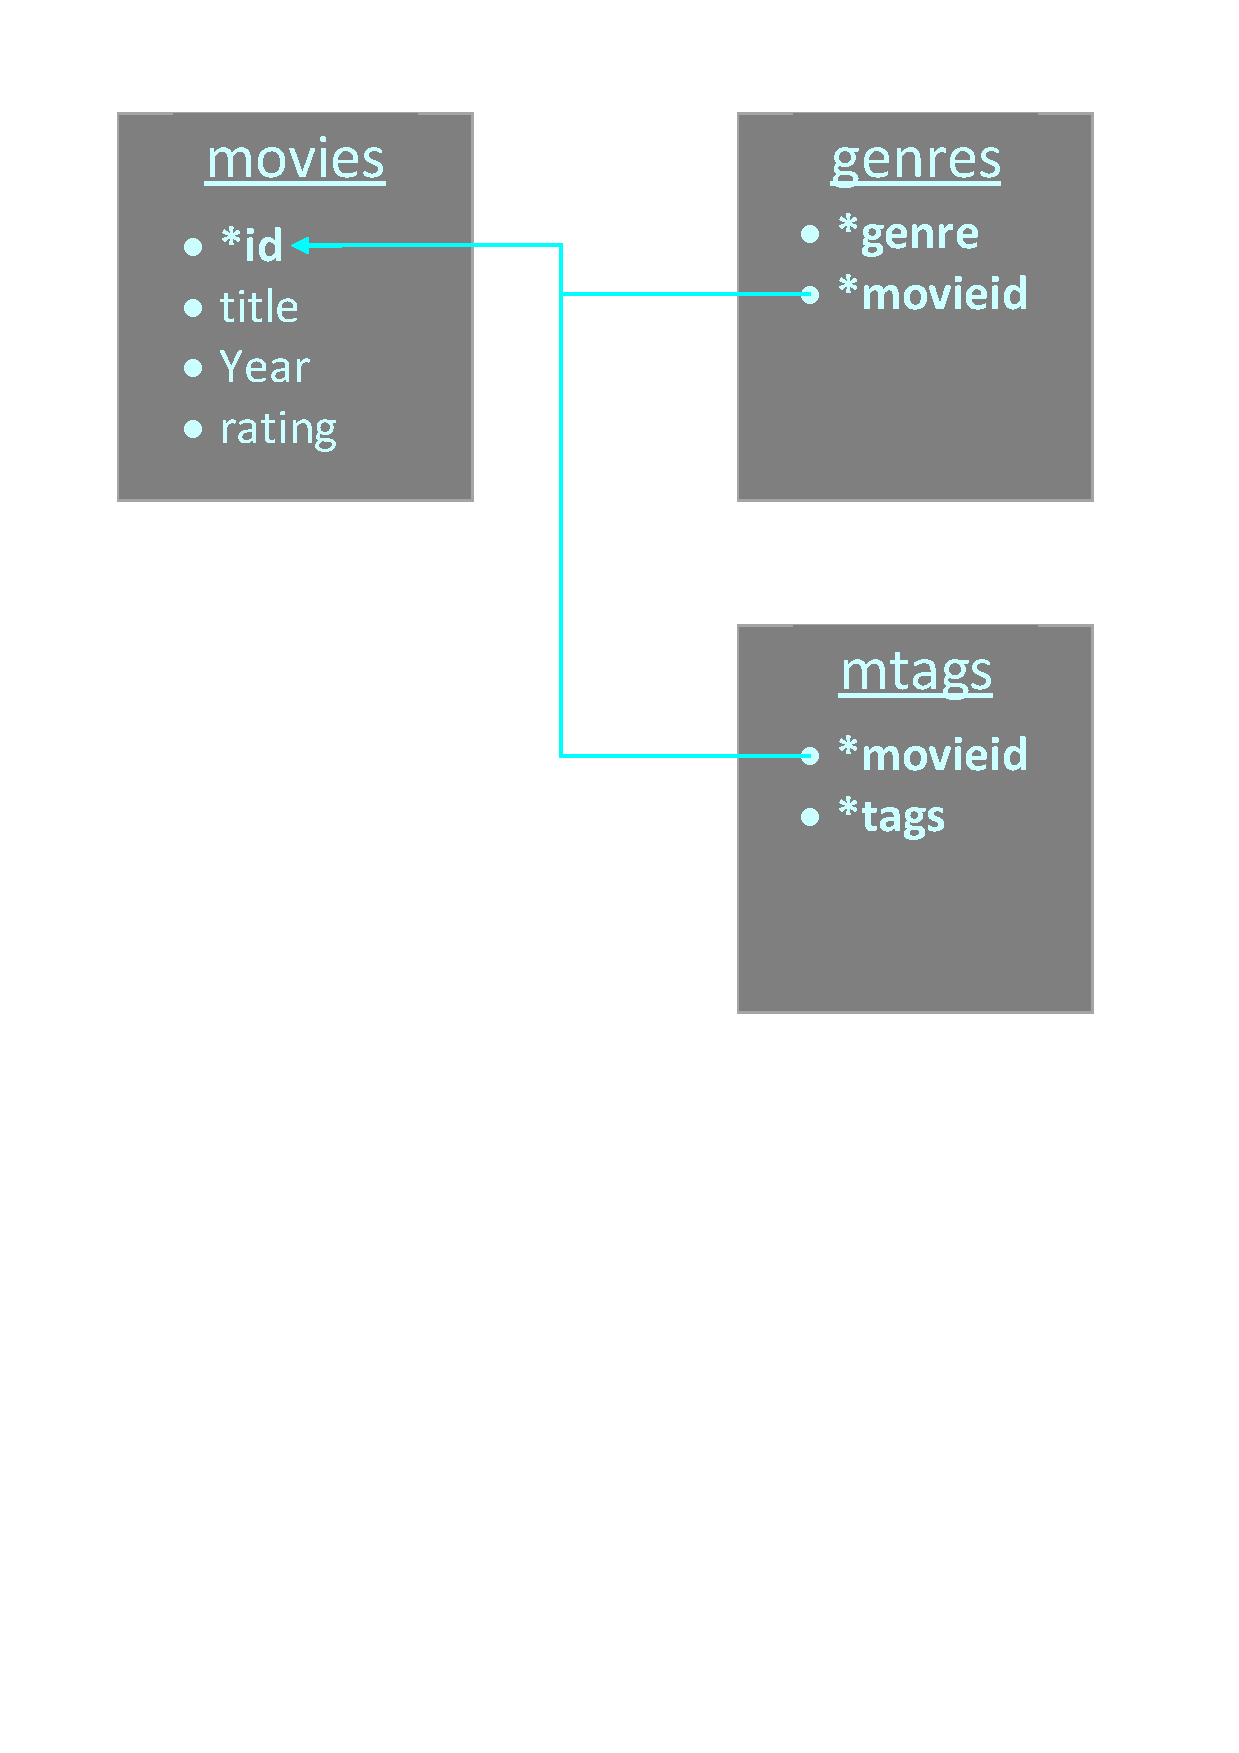
\includegraphics[width=\textwidth]{../graphics/ds.pdf}
	\caption{Database schema \label{fig:dataschema}}
\end{figure}

\begin{figure}
	\centering 
	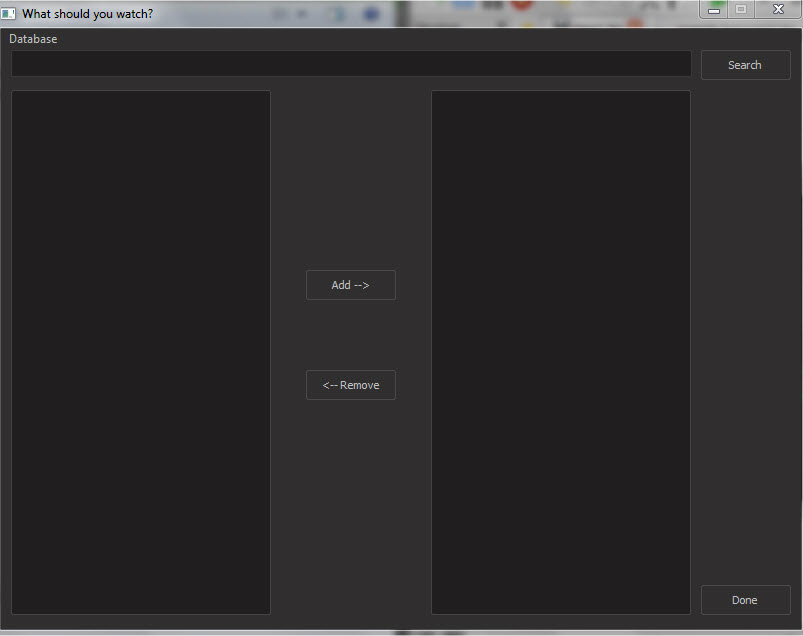
\includegraphics[width=\textwidth]{../graphics/cdbf.png}
	\caption{Sprettiglugginn \label{fig:cdbf}}
\end{figure}

\begin{figure}
	\centering 
	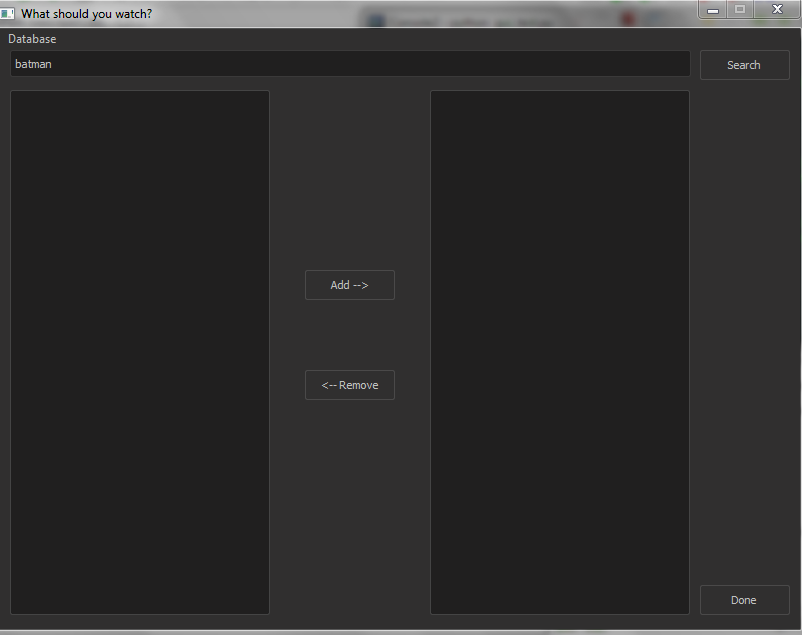
\includegraphics[width=\textwidth]{../graphics/dbf4.png}
	\caption{Sprettiglugginn \label{fig:dbf4}}
\end{figure}

\begin{figure}
	\centering 
	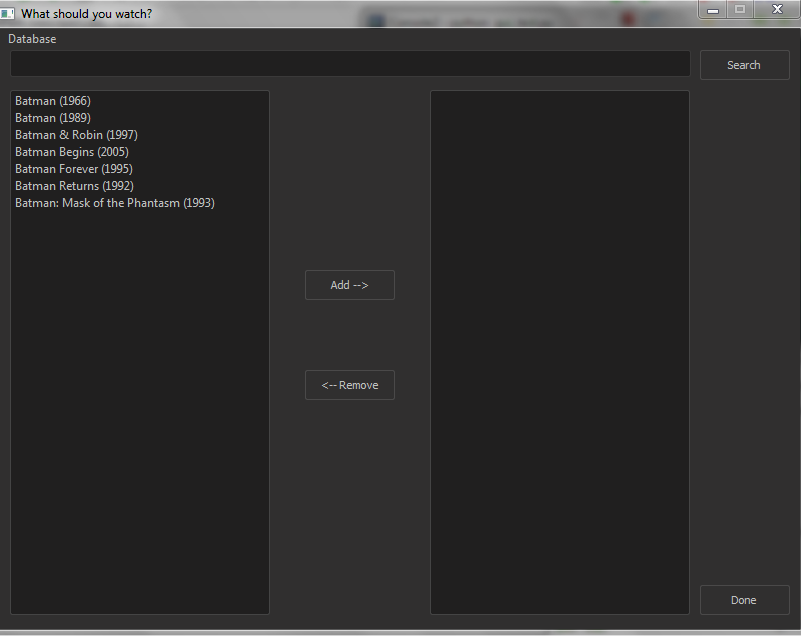
\includegraphics[width=\textwidth]{../graphics/dbf5.png}
	\caption{Sprettiglugginn \label{fig:dbf5}}
\end{figure}

\begin{figure}
	\centering 
	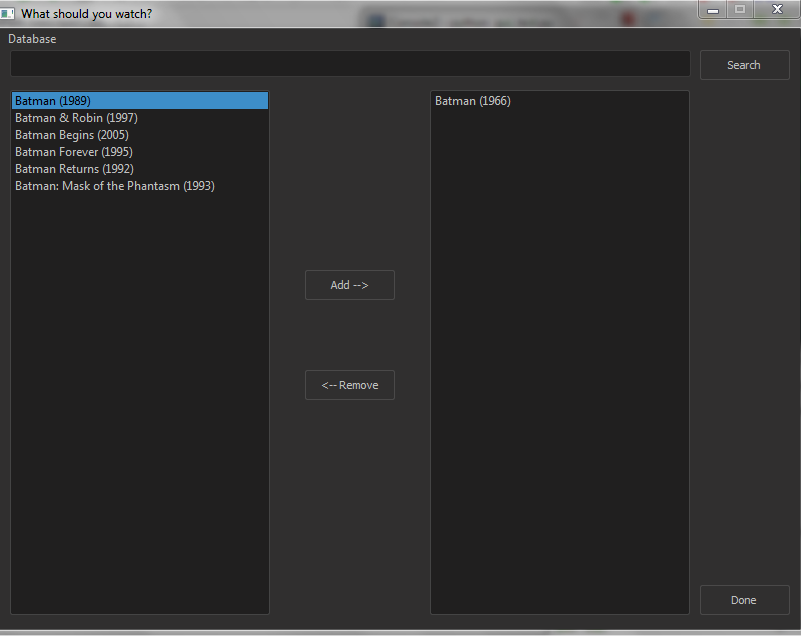
\includegraphics[width=\textwidth]{../graphics/dbf6.png}
	\caption{Sprettiglugginn\label{fig:dbf6}}
\end{figure}

\begin{figure}
	\centering 
	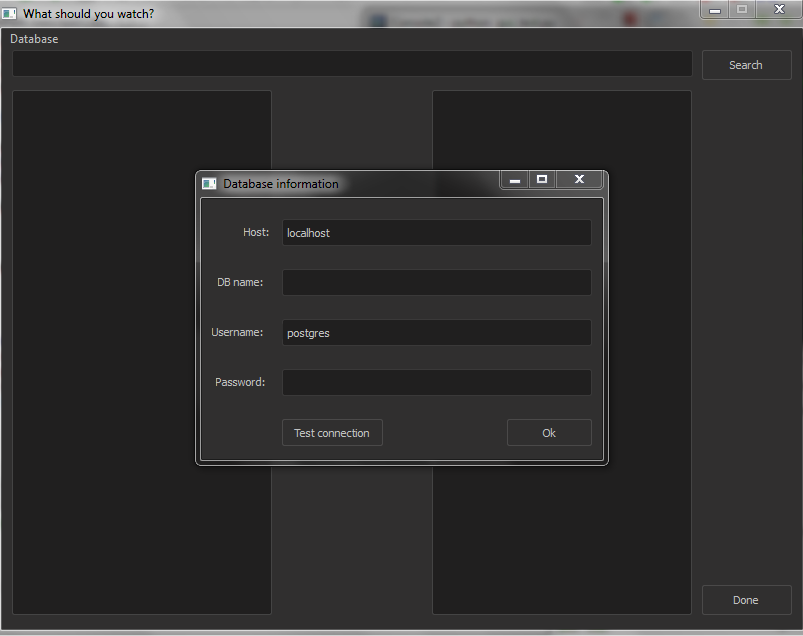
\includegraphics[width=\textwidth]{../graphics/dbf.png}
	\caption{Sprettiglugginn sem vantar upplýsingar  \label{fig:dbf}}
\end{figure}

\begin{figure}
	\centering 
	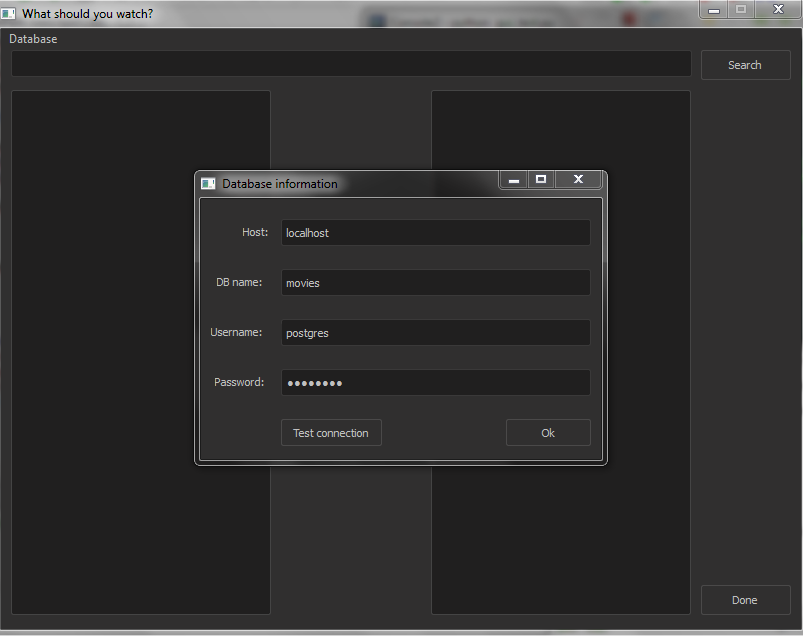
\includegraphics[width=\textwidth]{../graphics/dbf2.png}
	\caption{Sprettiglugginn með upplýsingum útfylltum \label{fig:dbf2}}
\end{figure}

\begin{figure}
	\centering 
	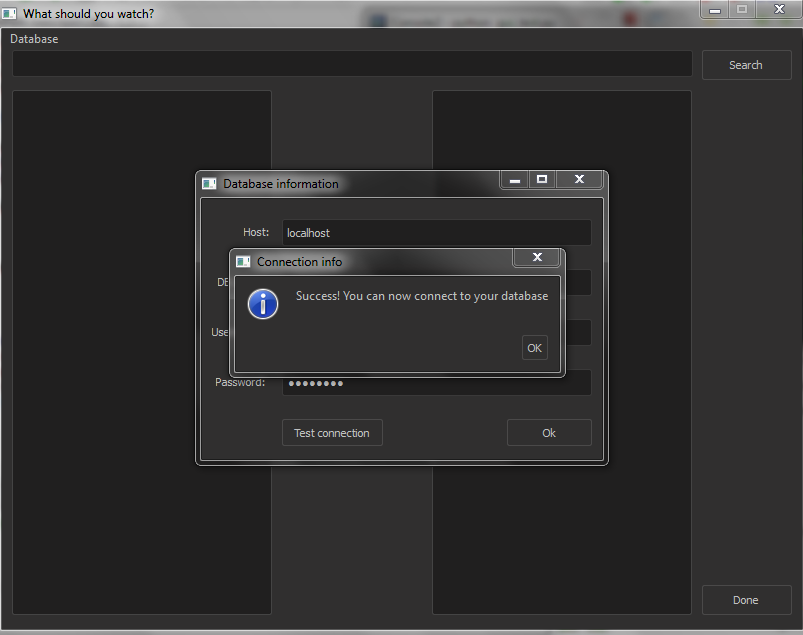
\includegraphics[width=\textwidth]{../graphics/pdf3.png}
	\caption{Sprettigluggin sem segir að tenging hafi tekist \label{fig:pdf3}}
\end{figure}

\begin{figure}
	\centering 
	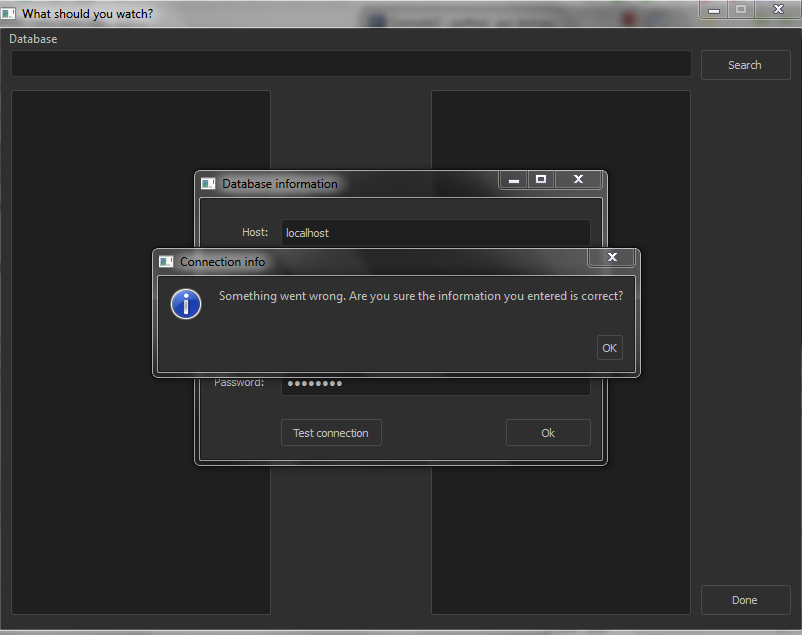
\includegraphics[width=\textwidth]{../graphics/dbf3.png}
	\caption{Sprettiglugginn sem segir að tenging hafi mistekist \label{fig:dbf3}}
\end{figure}



\clearpage
\printbibliography

\end{document} % this tells the compiler that we are done

% These are variables for the editor Emacs
%%% Local Variables: 
%%% TeX-command-BibTeX: biber
%%% mode: latex
%%% TeX-master: t
%%% End:
